
%%%%%%%%%%%%%%%%%%%%%%% file typeinst.tex %%%%%%%%%%%%%%%%%%%%%%%%%
%
% This is the LaTeX source for the instructions to authors using
% the LaTeX document class 'llncs.cls' for contributions to
% the Lecture Notes in Computer Sciences series.
% http://www.springer.com/lncs       Springer Heidelberg 2006/05/04
%
% It may be used as a template for your own input - copy it
% to a new file with a new name and use it as the basis
% for your article.
%
% NB: the document class 'llncs' has its own and detailed documentation, see
% ftp://ftp.springer.de/data/pubftp/pub/tex/latex/llncs/latex2e/llncsdoc.pdf
%
%%%%%%%%%%%%%%%%%%%%%%%%%%%%%%%%%%%%%%%%%%%%%%%%%%%%%%%%%%%%%%%%%%%


\documentclass[runningheads,a4paper]{llncs}

\usepackage{amssymb}
\setcounter{tocdepth}{3}
\usepackage{graphicx}
\usepackage{url}
\usepackage{amsmath}


\begin{document}

\mainmatter  % start of an individual contribution

% first the title is needed
\title{The Title of Your Thesis}

% a short form should be given in case it is too long for the running head
\titlerunning{Abbreviated Title of Your Thesis}

\author{Your Name(s)}
\institute{Your Field(s) of Study or Degree Program(s)\\
\email{name@domain.de}
}

%
% NB: a more complex sample for affiliations and the mapping to the
% corresponding authors can be found in the file "llncs.dem"
% (search for the string "\mainmatter" where a contribution starts).
% "llncs.dem" accompanies the document class "llncs.cls".
%

\toctitle{Lecture Notes in Computer Science}
\tocauthor{Authors' Instructions}
\maketitle


\begin{abstract}
Please include a brief summary of your thesis. It should definitely not exceed the space on the title page.
\keywords{Include some keywords that are representative of your thesis, e.g.: Privacy, Tracking, Tracking Technologies, Review}
\end{abstract}


\section{Introduction}
\label{section:intro}

In the introduction, you may want to address the following issues:
\begin{itemize}
	\item What is the overall topic space of your thesis?
	\item What is the specific problem area which you focus on? Why is it interesting, relevant, and/or otherwise worthy of study?
	\item Do you have concrete research questions which you pursue with your thesis?
	\item What is your approach and methodology to tackle this problem area and potentially your research questions? (For most of you this will be some form of review of the extant literature.)
	\item If suitable, can you give a brief summary/overview of your findings?
	\item Are there high-level takeaways for the topic space which you have targeted?
	\item Provide a very brief description of the structure of your thesis. (E.g.: In the following section, I/We will discuss ... Then, I/we will address... Finally, I/we will present a research idea based on my thesis work.)
	
\end{itemize}

\section{Paper Preparation in Latex}

\subsection{General Advice}

If you chose to work with Latex, then I assume you have some experience with this approach. You will need to use the files included in the zip file (in particular, Latex class \texttt{llncs.cls}), so that your text is typeset automatically in a uniform format. Please do not stray from the general layout of this template, except for good reason. Such reasons may include oversized figures and tables. If you are struggling with including such materials, then you can provide them also as separate files.

\subsection{Packages}

I have included already a package for URLs, which can be used as follows to, for example, refer to the site of the \textit{2017 Workshop on the Economics of Information Security}:  \url{http://weis2017.econinfosec.org/}. Of course, feel free to include further packages, which you may need for your thesis.

\subsection{Structure}

Please use sections and subsections as shown for this section to structure your thesis. 

\textbf{Detail:} Avoid subsubsections. Rather use bold font to further break down your text, as used in this case.

\subsection{Citations, References, and Footnotes}
\label{sub:citations}

To cite a paper please use the cite function as the following examples demonstrate:

Example 1 (Describe contents of a paper): Pu and Grossklags present an empirical study to investigate interdependent privacy preferences \cite{Pu2016}. 

Example 2 (Direct quote): Farhang and Grossklags expect their recent work on: ``Time-Based Security to positively impact the study of
security games of timing, as well as security practice.'' \cite{Farhang2017}.

The above citations are a journal article and a conference/workshop article, respectively. Here, is an example for a less formal reference like a reference to an institution \cite{CenterBiotech}. Here is a citation for a book \cite{Foster1999}.

The papers which I refer to are listed and formatted as bibitems below. Note that you would have to manually sort the items if you  want to have them in alphabetical order (or less recommended: in order of appearance). Also, if you include a bibitem in the list at the bottom of the file, it will be included in the references section irrespective whether you actually use it. So, please check at the end whether you do not have unneeded references included as bibitems. Personally, I use always separate bibliography files, and you are of course free to use this as well, if you are familiar with that approach.

Note, you can also refer to sections and subsections in your thesis. For example, I can point you to Section \ref{section:intro}, which is the introduction, or to Subsection \ref{sub:citations}, which is exactly this section. Note that you will have to label the sections with the \textit{label} command just below the item which you want to refer to.

Sometimes it is also useful to have footnotes to explain further details or to provide a definition etc.\footnote{This is how you would create a footnote.}

\subsection{Figures and Tables}

In the following, I will refer to the figure included in the Latex text below by properly labeling and referencing it.

Chancellor Merkel gave an informative speech at the dbb-Jahrestagung discussing the role and importance of digitalization in Germany. See, Figure\ref{fig:merkel} for a snapshot from the YouTube video available at: \url{https://www.youtube.com/watch?v=wNvJeoW7aVY}. 

\begin{figure}
\centering
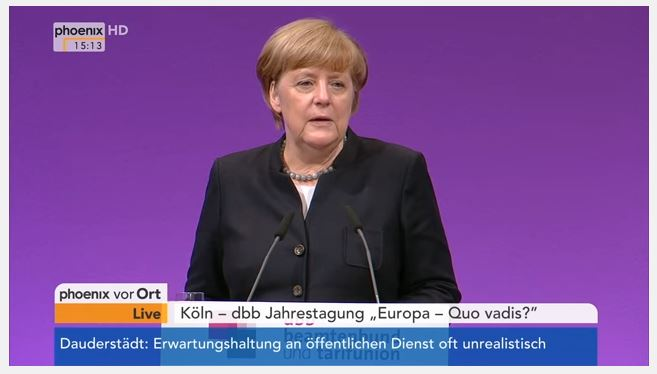
\includegraphics[height=6.2cm]{merkel}
\caption{Speech from Chancellor Merkel on January 9, 2017.}
\label{fig:merkel}
\end{figure}

Finally, I have included a table taken from \cite{Farhang2017} listing definitions of mathematical symbols. I would refer to the table in the text as Table \ref{table:symbols}.

 \begin{table}[t]
 	\centering
 	\caption{Summary of notations}\label{tab:Notation}
 	{\begin{tabular}{ll}
 			\hline
 			Variable & Definition \\
 			\hline
 			$\mathbf{p}$ & Protection time \\
 			$\mathbf{d}$ & Detection time \\
 			$\mathbf{r}$ & Reaction time \\
 			$c_{\mathbf{D}}$ & Defender's cost to reset the system's state \\
 			$c_\mathbf{k}$  & Defender's cost to check the state of the system \\
 			$c_{\mathbf{A}}$ & Attacker's cost to compromise the defender \\
 			$t_\mathbf{D}$ & Time between two consecutive checks by the defender \\
 			$t_{\mathbf{A}}$ & Time between two consecutive moves by the attacker \\
 			$\tau_{\mathbf{D}}$ & Average fraction of time that the defender controls the resource \\
 			$\delta_{\mathbf{D}}$ & Average time between the defender's two consecutive reset moves \\
 			$u_{\mathbf{D}}$ & Defender's utility \\
 			$u_{\mathbf{A}}$ & Attacker's utility \\
 			\hline
 		\end{tabular}
 	}
 	\label{table:symbols}
 \end{table}

\section{Good Luck!}

Please feel free to contact me with any further questions. Otherwise, good luck with completing your seminar thesis in Latex.

\begin{thebibliography}{4}

\bibitem{Pu2016} Pu, Yu, and Grossklags, Jens: Towards a Model on the Factors Influencing Social App Users' Valuation of Interdependent Privacy. Proceedings on Privacy Enhancing Technologies, Volume 2016, Number 2, pages 61-81 (2016)

\bibitem{Foster1999} Foster, I., Kesselman, C.: The Grid: Blueprint for a New Computing
Infrastructure. Morgan Kaufmann, San Francisco (1999)

\bibitem{Farhang2017} Farhang, Sadegh, and Grossklags, Jens: When to Invest in Security? Empirical Evidence and a
Game-Theoretic Approach for Time-Based Security. Workshop on the Economics of Information Security (2017)

\bibitem{CenterBiotech} National Center for Biotechnology Information, \url{http://www.ncbi.nlm.nih.gov}

\end{thebibliography}


\section*{Checklist of Items to be Sent to Seminar Instructor}
Here is a checklist of everything I require from you:


\begin{itemize}
\settowidth{\leftmargin}{{\Large$\square$}}\advance\leftmargin\labelsep
\itemsep8pt\relax
\renewcommand\labelitemi{{\lower1.5pt\hbox{\Large$\square$}}}

\item The final \LaTeX{} source files as a ZIP file
\item A final PDF file

\end{itemize}
\end{document}
